\documentclass[twocolumn]{jarticle}
\usepackage{jsaiac}
\usepackage{color}
\usepackage[dvipdfmx]{graphicx}
\usepackage{amsmath}
\usepackage{amssymb}
\usepackage{multirow}
\usepackage{url}
\usepackage{bm}
\usepackage{here}

%%
\title{
\jtitle{知的学習システム第2回レポート}
}
%%英文は以下を使用
%\title{Style file for manuscripts of JSAI 20XX}

%\jaddress{岡本 一志,電気通信大学 大学院情報理工学研究科 情報学専攻,東京都調布市調布ヶ丘1-5-1,Tel.: 042-443-5280,E-mail: kazushi@uec.ac.jp}

\author{%
\jname{1930099 服部 凌典}
}

\affiliate{
\jname{電気通信大学 大学院情報理工学研究科 情報学専攻}
}

%%
%\Vol{28}        %% <-- 28th(変更しないでください)
%\session{0A0-00}%% <-- 講演ID(必須)

%\setcounter{page}{1}
\def\Style{``jsaiac.sty''}
\def\BibTeX{{\rm B\kern-.05em{\sc i\kern-.025em b}\kern-.08em%
 T\kern-.1667em\lower.7ex\hbox{E}\kern-.125emX}}
\def\JBibTeX{\leavevmode\lower .6ex\hbox{J}\kern-0.15em\BibTeX}
\def\LaTeXe{\LaTeX\kern.15em2$_{\textstyle\varepsilon}$}

\begin{document}
\maketitle


\section{課題1}
1変数ガウス分布の対数尤度関数の最大値を与えるパラメータは
\begin{eqnarray}
\mu=\dfrac{1}{N} \displaystyle\sum_{n=1}^{N}x_n\end{eqnarray}

\begin{eqnarray}
\sigma^2=\dfrac{1}{n}\displaystyle\sum_{k=1}^n(x_k-\mu)^2
\end{eqnarray}
のときである.

\section{課題2}
1変数ポアソン分布のパラメータ$\lambda$の最尤推定量は,$\{x_1, x_2, \cdots, x_n\}$の平均値である
\begin{eqnarray}
\lambda =\dfrac{1}{N} \displaystyle\sum_{n=1}^{N}x_n
\end{eqnarray}

のときである.

\section{課題3}
図1-3に標準正規分布に従う$\{10, 100, 1000, 10000\}$個の4通りの乱数のヒストグラムを示す.
また,それぞれの個数で3回づつ乱数を生成している.
図4-6は図1-3からそれぞれ最尤推定によって,パラメータを推定した結果の図である。
また,表1は図1-3に対応するそれぞれの平均を示した表である.
表1と,図1-3から生成する乱数を増やすごとに平均が$0$に近づくことを確認している.
また,$\{10, 100, 1000, 10000\}$個の乱数を生成するものにおいて,それぞれで3回の試行による平均の分散は$\{10, 100, 1000, 10000\}$の順に$\{0.19, 0.27\times 10^{-1}, 0.62\times 10^{-3}, 0.9 \times 10^{-7}\}$となり,生成する乱数を増やすごとに試行毎の平均のばらつきが減少することを確認している.
加えて,1000個の乱数を生成したものと10000個の乱数を生成したものでは,表1から平均値に違いは見られなかったが,図3-4より,10000個の乱数を生成したものの方が標準正規分布の形に近いと考える.
また,図1-6により,100個以上の乱数を生成するものが最尤推定から求めた正規分布とヒストグラムの形状が近いことが確認できる.

\begin{table}[t]
  \begin{center}
      \caption{NとMに対応するMSE}
    \label{table1}
\begin{tabular}{llll}
  & 10   & 100  & 1000 \\
2 & 0.85 & 0.63 & 0.62 \\
4 & 0.85 & 0.63 & 0.62 \\
8 & 0.85 & 0.63 & 0.62
\end{tabular}
\end{center}
\end{table}
\begin{figure}[h]
  \begin{center}
    \begin{tabular}{ccc}
      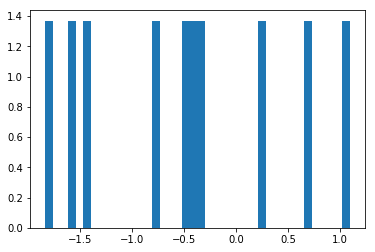
\includegraphics[width=0.32\hsize]{figure/10_1.png} &
      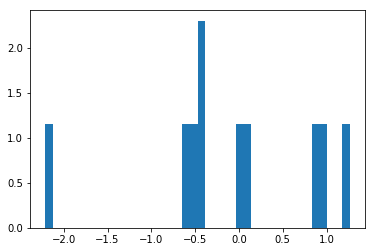
\includegraphics[width=0.32\hsize]{figure/10_2.png} &
      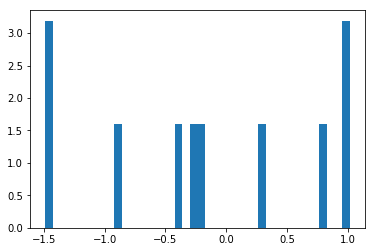
\includegraphics[width=0.32\hsize]{figure/10_3.png} \\
      試行1 & 試行2 &試行3
    \end{tabular}
    \caption{標準正規分布に基づく10個の乱数のヒストグラム}
    \label{figure1}
  \end{center}
\end{figure}
\begin{figure}[h]
  \begin{center}
    \begin{tabular}{ccc}
      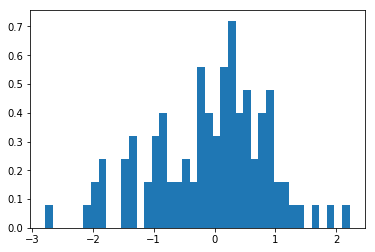
\includegraphics[width=0.32\hsize]{figure/100_1.png} &
      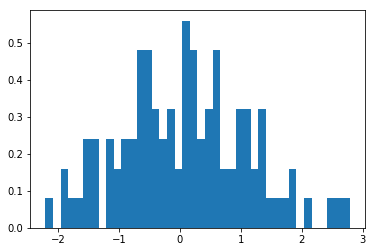
\includegraphics[width=0.32\hsize]{figure/100_2.png} &
      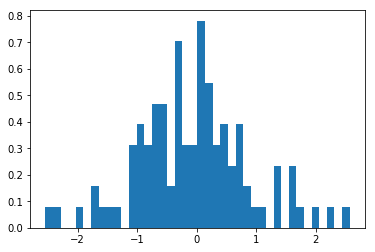
\includegraphics[width=0.32\hsize]{figure/100_3.png} \\
      試行1 & 試行2 &試行3
    \end{tabular}
    \caption{標準正規分布に基づく100個の乱数のヒストグラム}
    \label{figure1}
  \end{center}
\end{figure}
\begin{figure}[h]
  \begin{center}
    \begin{tabular}{ccc}
      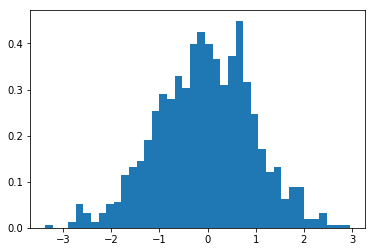
\includegraphics[width=0.32\hsize]{figure/1000_1.png} &
      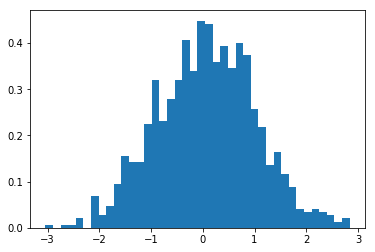
\includegraphics[width=0.32\hsize]{figure/1000_2.png} &
      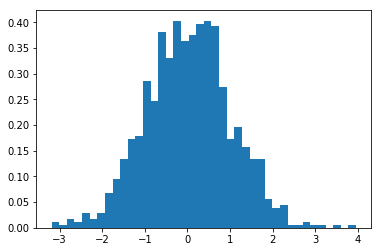
\includegraphics[width=0.32\hsize]{figure/1000_3.png} \\
      試行1 & 試行2 &試行3
    \end{tabular}
    \caption{標準正規分布に基づく1000個の乱数のヒストグラム}
    \label{figure1}
  \end{center}
\end{figure}
\begin{figure}[h]
  \begin{center}
    \begin{tabular}{ccc}
      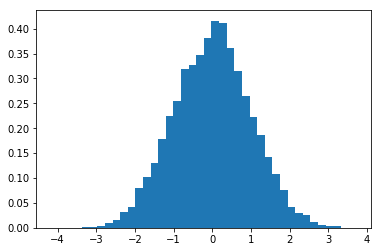
\includegraphics[width=0.32\hsize]{figure/10000_1.png} &
      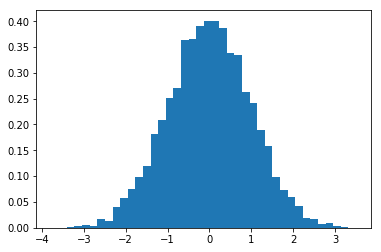
\includegraphics[width=0.32\hsize]{figure/10000_2.png} &
      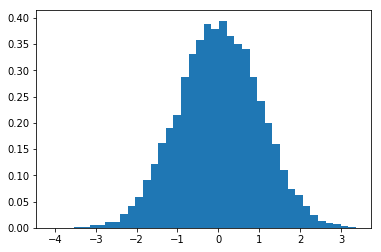
\includegraphics[width=0.32\hsize]{figure/10000_3.png} \\
      試行1 & 試行2 &試行3
    \end{tabular}
    \caption{標準正規分布に基づく10000個の乱数のヒストグラム}
    \label{figure1}
  \end{center}
\end{figure}

\begin{figure}[h]
  \begin{center}
    \begin{tabular}{ccc}
      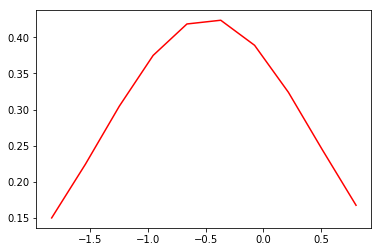
\includegraphics[width=0.32\hsize]{figure/10__1.png} &
      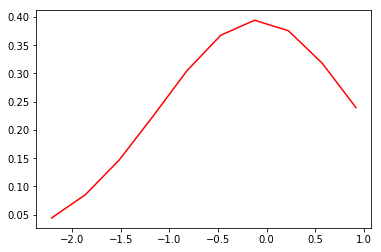
\includegraphics[width=0.32\hsize]{figure/10__2.png} &
      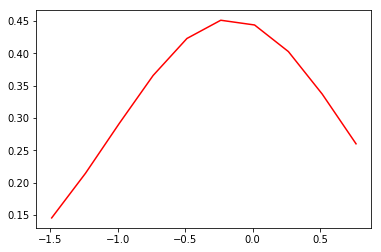
\includegraphics[width=0.32\hsize]{figure/10__3.png} \\
      試行1 & 試行2 &試行3
    \end{tabular}
    \caption{標準正規分布に基づく10個の乱数の分布}
    \label{figure1}
  \end{center}
\end{figure}
\begin{figure}[h]
  \begin{center}
    \begin{tabular}{ccc}
      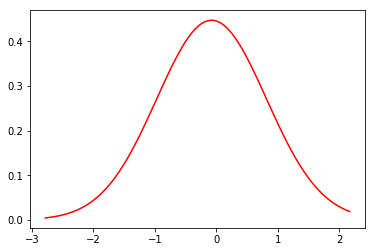
\includegraphics[width=0.32\hsize]{figure/100__1.png} &
      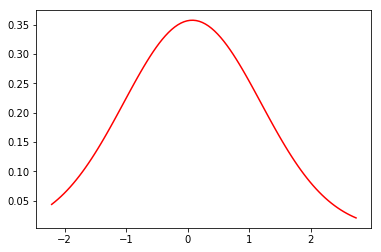
\includegraphics[width=0.32\hsize]{figure/100__2.png} &
      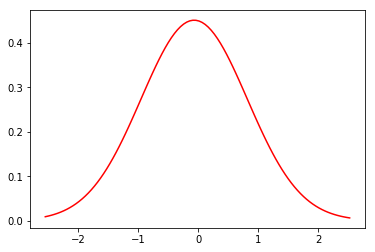
\includegraphics[width=0.32\hsize]{figure/100__3.png} \\
      試行1 & 試行2 &試行3
    \end{tabular}
    \caption{標準正規分布に基づく100個の乱数の分布}
    \label{figure1}
  \end{center}
\end{figure}
\begin{figure}[h]
  \begin{center}
    \begin{tabular}{ccc}
      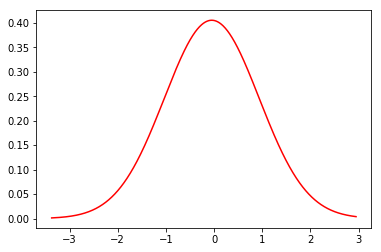
\includegraphics[width=0.32\hsize]{figure/1000__1.png} &
      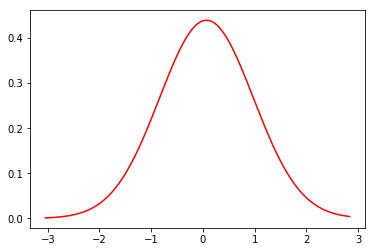
\includegraphics[width=0.32\hsize]{figure/1000__2.png} &
      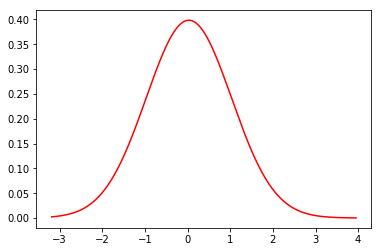
\includegraphics[width=0.32\hsize]{figure/1000__3.png} \\
      試行1 & 試行2 &試行3
    \end{tabular}
    \caption{標準正規分布に基づく1000個の乱数の分布}
    \label{figure1}
  \end{center}
\end{figure}
\begin{figure}[h]
  \begin{center}
    \begin{tabular}{ccc}
      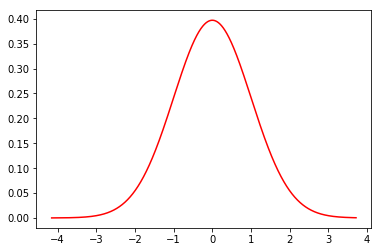
\includegraphics[width=0.32\hsize]{figure/10000__1.png} &
      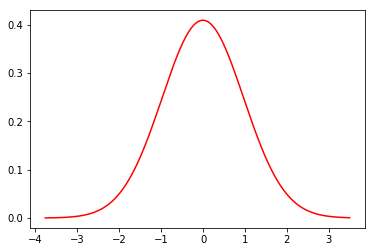
\includegraphics[width=0.32\hsize]{figure/10000__2.png} &
      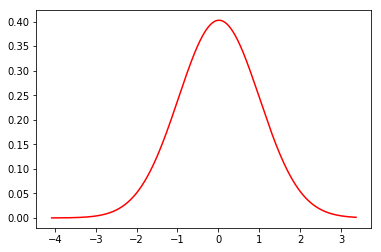
\includegraphics[width=0.32\hsize]{figure/10000__3.png} \\
      試行1 & 試行2 &試行3
    \end{tabular}
    \caption{標準正規分布に基づく10000個の乱数の分布}
    \label{figure1}
  \end{center}
\end{figure}


\end{document}
